\documentclass[a4paper, oneside, openany, dvipsnames, table, 12pt]{article}
\usepackage{../Template/AFKstyle}
\usepackage{hyperref}
\usepackage{amsmath}
\newcommand{\Titolo}{Verbale esterno 2020-03-31}

\newcommand{\Gruppo}{TeamAFK}

\newcommand{\Redattori}{Simone Meneghin}

\newcommand{\Verificatori}{z}

\newcommand{\pathimg}{../../Template/img/logoAFK.png}

\newcommand{\Approvatore}{a}

\newcommand{\Distribuzione}{Prof. Vardanega Tullio \newline Prof. Cardin Riccardo \newline TeamAFK}

\newcommand{\Uso}{Esterno}

\newcommand{\NomeProgetto}{"Predire in Grafana"}

\newcommand{\Mail}{gruppoafk15@gmail.com}

\newcommand{\Versionedoc}{1.0.0}

\newcommand{\DescrizioneDoc}{Riassunto dell'incontro del gruppo \textit{TeamAFK} con il proponente tenutosi il 2020-03-31.}


\makeindex

\begin{document}
\copertina{}

%definizione colori per tabelle (tranne copertina)
\definecolor{redafk}{RGB}{255, 71, 87}
\definecolor{grey2}{RGB}{204, 204, 204}
\definecolor{greyRowafk}{RGB}{234, 234, 234}
\rowcolors{2}{grey2}{greyRowafk}
\renewcommand{\arraystretch}{1.5}

\newpage
\section*{Registro delle modifiche}
{
	\centering
	\begin{longtable}{ c c  C{4cm}  c  c }
		\rowcolor{redafk}
		\textcolor{white}{\textbf{Versione}} & \textcolor{white}{\textbf{Data}} & \textcolor{white}{\textbf{Descrizione}} & \textcolor{white}{\textbf{Nominativo}} & \textcolor{white}{\textbf{Ruolo}}\\		
		0.0.1 & 2020-03-20 & Stesura documento & Davide Zilio &\reda{}\\		
		
	\end{longtable}

}

%Didascalia tabelle/immagini (prendono come riferimento la subsection)
\counterwithin{table}{subsection}
\counterwithin{figure}{subsection}
\newpage

%indice, indice figure e indice tabelle
\tableofcontents
\newpage
\listoffigures
\newpage
\listoftables
\newpage

\section{Introduzzione}
\subsection{Premessa}
Il \textit{Piano di Qualifica} è un documento su cui si prevede di lavorare l'intera durata del progetto. Molti dei contenuti del documento sono di natura instabile. Ad esempio, molte delle metriche scelte non sono applicabili nella fase iniziale, e solo con il loro utilizzo pratico si può valutarne l'effettiva utilità. Anche i processi selezionati possono essere soggetti a cambiamenti, rivelandosi insufficienti o inadeguati agli scopi del progetto e al modo di lavorare del team. Il documento è stato scritto in diversi periodi in quanto alcune delle cose non le si potevano conoscere a priori. \\
Per tutte queste ragioni, il documento è prodotto in maniera incrementale, e i suoi contenuti iniziali sono da considerarsi incompleti: subiranno significative aggiunte e modifiche nel tempo.

\subsection{Scopo del documento}
Questo documento ha lo scopo di mostrare le strategie di verifica\glo e validazione\glo adottate al fine di garantire la qualità di prodotto e di processo. Per raggiungere questo obiettivo viene applicato un sistema di verifica continua sui processi in corso e sulle attività svolte. In questo modo è quindi possibile rilevare e correggere all'istante eventuali anomalie, riducendo al minimo lo spreco delle risorse.

\subsection{Scopo del prodotto}
Lo scopo del prodotto è quello di realizzare due plug-in per il software Grafana\glo, che permettano di monitorare e predire lo stato di un sistema in analisi. Grazie alle predizioni sarà possibile attivare degli allarmi così da poter gestire preventivamente eventuali situazioni di rischio. \\
I due plug-in\glo utilizzeranno la Support Vector Machine\glo (SVM) per poter effettuare regressione lineare o categorizzazione sui dati forniti.

\subsection{Glossario}
Per evitare ambiguità nei documenti formali, viene fornito il documento \textbf{Glossario},
contenente tutti i termini considerati di difficile comprensione. Perciò nella documentazione fornita, ogni vocabolo contenuto in Glossario è contrassegnato dalla lettera G a pedice.

\subsection{Riferimenti}
\subsubsection{Riferimenti normativi}
\begin{itemize}
	\item \textit{Norme di Progetto};
	\item ISO/IEC 9126: \\
	https://en.wikipedia.org/wiki/ISO/IEC_9126
	\item ISO/IEC 15504: \\
	https://en.wikipedia.org/wiki/ISO/IEC_15504
\end{itemize}
\subsubsection{Riferimenti informativi}
\begin{itemize}
	\item Capitolato d'appalto C4: \\
	 https://www.math.unipd.it/~tullio/IS-1/2019/Progetto/C4.pdf
\end{itemize}
\pagebreak

\section{Processi primari}
	\subsection{Fornitura}
		\subsubsection{Scopo}
		Lo scopo del processo di fornitura consiste nelle attività e compiti dell'acquirente, come risposta ai bisogni del cliente in ambito di sistema, prodotto e/o servizio software. Nello specifico, le caratteristiche richieste dal proponente sono analizzate e stilate nello \textit{Studio di Fattibilità}, il quale è alla base del processo di fornitura. Dopodiché è possibile stabilire le risorse e le procedure necessarie alla redazione di un \textit{Piano di Progetto} da seguire fino alla consegna del materiale prodotto.
		Nel dettaglio le attività svolte da questo processo sono:
		\begin{itemize}
			\item avvio;
			\item studio di fattibilità;
			\item contrattazione;
			\item progettazione;
			\item esecuzione e controllo;
			\item revizione e valutazione;
			\item consegna e completamento.
		\end{itemize}
		\subsubsection{Aspettative}
		Il gruppo deve avere un frequente contatto con il cliente al fine di rispettare i vincoli obbligatori da lui fissati, onde evitare di scostarsi troppo dal prodotto finale richiesto. Per questo è necessario comunicare con il proponente, per poter aver chiari i bisogni che tale prodotto intende soddisfare con le sue funzionalità.
		Quindi, ogni qualvolta il gruppo venga a contatto con il proponente, deve stabilire:
		\begin{itemize}
			\item aspetti chiave che soddisfano i bisogni richiesti;
			\item requisiti e vincoli dei processi;
			\item verifica continua;
			\item chiarimento di eventuali dubbi;
			\item accordo sulla qualifica del prodotto;
			\end{itemize} 
		\subsubsection{Descrizione}
		Questa sezione ha il compito mostrare le norme che \textit{TeamAFK}, in tutte le attività di progettazine, sviluppo e consegna del prodotto \textit{Predire in Grafana}, con lo scopo di diventare fornitori del capitolato  dal proponente \textit{Zucchetti SPA} e dai committenti Prof. Tullio Vardanega e Prof. Riccardo Cardin.
		\subsubsection{Attività}
			\paragraph{Studio di Fattibilità} \mbox{} \\ \mbox{} \\
			Lo \textit{Studio di Fattibilità}, redatto per ogni capitolato\glo dagli analisti illusttra:
			\begin{itemize}
				\item \textbf{Descrizione generale}: sintesi delle informazioni generali del capitolato, e delle circostanze da cui sorgono tali richieste;
				\item \textbf{Obiettivi}: vengono mostrate le caratteristiche principali del prodotto e i relativi obiettivi da raggiungere;
				\item \textbf{Tecnologie utlizzate}: corrisponde all'elenco degli strumenti messi a disposizione dall'azienda proponente al team per sviluppare il progetto;
				\item \textbf{Valutazione finale}: si tratta di un commento elaborato dal gruppo, una volta riunitosi e analizzato le  richieste dell'azienda, motivando la scelta di focalizzarsi o meno su una determinata offerta.
			\end{itemize}

			\paragraph{Piano di Progetto} \mbox{} \\ \mbox{} \\
			Il \textit{Piano di Progetto} un documento redatto dal progect manager\glo e dagli amministratori, e si aggiunge all'insieme dei documenti che il team dovrà seguire per tutta la durata del progetto. In particolare questo documento conterrà:
			\begin{itemize}
				\item \textbf{Analisi dei rischi}: il fornitore analizza tutti gli eventuali rischi di tipo tecnico, economico e temporale che possono presentarsi durante il progetto, fornendo anche soluzioni che possano risolverli o almeno limitare i loro effetti negativi;
				\item \textbf{Modello di sviluppo}\glo: viene definita la struttura su cui basarsi per la pianificazione, esecuzine e consegna del prodotto software;
				\item \textbf{Pianificazione}: viene pianificato l'insieme delle attività da eseguire durante le fasi di progetto, collocandole nel tempo e stabilendo le loroo scdenze;
				\item \textbf{Preventivo e consuntivo}: con il preventivo viene mostrata una stima di quello che sarà il carico di lavoro che il team sosterrà durante il progetto, in termini di tempo e i relativi costi. Con il consuntivo di periodo, invece verranno riportati le variazioni dei costi rispetto a quanto preventivato.
			\end{itemize}

			\paragraph{Piano di Qualifica} \mbox{} \\ \mbox{} \\
			I verificatori si occuperanno di redigere il \textit{Piano di Qualifica}. Ovvero l'insieme di attività con il compito di fissare obiettivi di qualità del prodotto nel suo complesso. Quindi considerando anche i processi e le risorse necessarie a raggiungere tali obiettivi. Nel dettaglio il \textit{Piano di Qualifica} si focalizza su:
			\begin{itemize}
				\item \textbf{Qualità di prodotto}: vengono fissate le politiche per il raggiungimento della qualità, gli obiettivi da raggiungere e gli strumenti necessari al controllo;
				\item \textbf{Qualità di processo}: stabilire sulla base di opportune misurazioni, il grado di efficacia ed efficenza di un processo a partire dalla sua definizione;
				\item \textbf{Standard di qualità}: vengono selezionati gli standard che verranno seguiti, per garantire la stabilità del prodotto;
				\item \textbf{Valutazione di miglioramento}: i problemi e le relative soluzioni vengono evidenziate in questa sezione del \textit{Piano di Qualifica};
				\item \textbf{Resoconto dell'attività di verifica}: vengono riportate i risultati delle metriche come resoconto dell'attività di qualifica.
			\end{itemize}
		\subsubsection{Strumenti}
		Di seguito sono illustrati gli strumenti utilizzati per lo svolgimento dell'attivita di fornitura.

	\subsection{Sviluppo}
		\subsubsection{Scopo}Questo è il processo che si occupa di stabilire le attività da svolgere per costruire e consegnare il prodotto finale.
		\subsubsection{Aspettative}
		Le aspettative sono le seguenti:
			\begin{itemize}
				\item stabilire obiettivi di sviluppo;
				\item stabilire vincoli tecnici;
				\item stabilire vincoli di design;
				\item realizzare il prodotto software che superi i test, e soddisfi i vincoli di progetto.
			\end{itemize}
		\subsubsection{Descrizione}
			Il processo di sviluppo si divide in:
				\begin{itemize}
					\item \textit{Analisi dei Requisiti};
					\item Progettazione;
					\item Codifica.
				\end{itemize}
		\subsubsection{Attività}
			\paragraph{Analisi dei Requisiti} \mbox{} \\ \mbox{} \\
			L'elenco dei requisiti necessari allo svolgimento de processo di sviluppo, viene raccolto e redatto dagli analisti in un apposito documento di \textit{Analisi dei Requisiti}. Quest'ultimo ha lo scopo di:
				\begin{itemize}
					\item Scopo del prodotto;
					\item Fornire ai progettisti riferimenti precisi ed affidabili;
					\item Stabilire le prospettive e funzionalità del prodotto in base ai vincoli fissati dal proponente;
					\item Fornire ai verificatori riferimenti affidabili per la loro attività di controllo;
					\item Valutare rischi, costi e benefici in relazione al carico di lavoro.
				\end{itemize} 
			\subparagraph*{Aspettative} \mbox{} \\ \mbox{} \\
			L'obiettivo di quest'attività è quella di redigere un documento formale contenente tutti requisiti che richiesti dal progetto.
			\subparagraph*{Descrizione} \mbox{} \\ \mbox{} \\
			I requisiti saranno raccolti nel seguente modo:
				\begin{itemize} 
					\item lettura del capitolato d'appalto;
					\item confronto con il proponente;
					\item discussione tra i componenti del gruppo;
					\item studio di casi d'uso.
				\end{itemize}
				\subparagraph*{Casi d'uso} \mbox{} \\ \mbox{} \\
				I casi d'uso sono scenari che descrivono una possibile sequenza di iterazioni dell'utente, visto come attore\glo attivo e/o passivo, e il sistema. La struttura di un caso d'uso è la seguente:
				\begin{itemize}
					\item codice identificativo;
					\item titolo;
					\item diagramma UML\glo;
					\item attori primari;
					\item attori secondari;
					\item descrizione;
					\item scenario principale;
					\item scenario alternativo (se presente);
					\item inclusioni (se presenti);
					\item estensioni (se presenti);
					\item specializzazioni (se presenti);
					\item precondizione;
					\item postcondizione. 
				\end{itemize}
				\subparagraph*{Codice identificativo dei casi d'uso} \mbox{} \\ \mbox{} \\
			Il codice di ogni caso d'uso seguirà questo formalismo: \newline \newline
			\centerline{\textbf{UC[codice\_padre].[codice\_figlio]}} \newline \newline
			\textbf{Requisiti} \newline \newline
			I requisiti seguiranno la seguente struttura:
				\begin{itemize}
					\item \textbf{codice identificativo}: è un codice univoco e conforme alla codifica: \newline \newline
					\centerline{\textbf{R[Importanza][Tipologia][Codice]}} \newline \newline
					Le voci riportate nella precedente codifica significano: 
					\begin{itemize}
						\item \textbf{Importanza}: la quale può assumere come valori:
						\begin{itemize}
							\item 1: requisito obbligatorio, irrinuunciablie;
							\item 2: requisito desiderabile, perciò non obbligatorio ma riconosscibile;
							\item 3: requisito opzionale, ovvero trattabile in un secondo momento o relativamente utile.
						\end{itemize}
						\item \textbf{Tipologia}: la quale può assumere come valori:
						\begin{itemize}
							\item F: funzionale;
							\item P: prestazionale;
							\item Q: qualitativo;
							\item V: vincolo.
						\end{itemize}
						\item \textbf{Codice identificativo}: il quale è un identificatore univoco del requisito, e viene espresso in forma gerarchica padre/figlio.
					\end{itemize}
					\item \textbf{Classificazione}: specifica il peso del requisito facilitando la sua lettura anche se causa ridondanza;
					\item \textbf{Descrizione}: sintei completa di un requisito;
					\item \textbf{Fonti}: il requisito può avere le seguenti provenienze:
					\begin{itemize}
						\item capitolato;
						\item interno: requisito che gli analisti ritengono di aggiungere in base alle esigenze del team;
						\item caso d'uso: il requisito proviene da uno o più casi d'uso, dei quali è necessario riportare il codice univoco di caso d'uso;
						\item verbale: dopo un chiarimento da parte del proponente è possibile che sorga un requisito non preventivato. E le informazioni su di esso sono riportate e tracciati nei rispettivi verbali.
					\end{itemize}
				\end{itemize} 
				\subparagraph*{UML} \mbox{} \\ \mbox{} \\
				I diagrammi UML\glo servono per descrivere un caso d'uso. Gli analisti dovranno utilizzare la versione v.2.0. \newline \newline
	\subsection{Progettazione}
		\subsubsection{Scopo}
		Il processo di \textit{Progettazione} ha il copito di stabilire le migliori operazioni da effettuare, per fornire una soluzione soddisfacente per tutti gli stakeholders\glo. Per far ciò è necessario stabilire l'architettura\glo logica del prodotto. Sulla base del documento \textit{Analisi dei Requisiti} è possibile individuare le singole parti che compongono il prodotto, il loro dominio e una complessità trattabile. Una volta avute ben chiare queste peculiarità, sarà possibile determinare l'architettura del prodotto.
		\subsubsection{Descrizione}
		Il processo di \textbf{Progettazione} si divide in:
			\begin{itemize}
				\item \textbf{Technology baseline}: mostra ad alto le specifiche di progettazione del prodotto e le sue componenti, elencando i diagrammi UML utilizzati per descrivere l'architettura delprodotto.
				\item \textbf{Product baseline}: parte incrementale del prodotto finale da cui continuare a lavorare, integrando le specifiche riportate nella Tecnology Baseline e  definendo anche i test necessari alla verifica.
			\end{itemize} 
			\paragraph{Technology baseline} \mbox{} \\ \mbox{} \\
			Il progettista incaricato, si occuperà di includere:
			\begin{itemize}
				\item \textbf{Diagrammi UML}:
				\begin{itemize}
					\item diagrammi delle classi;
					\item diagrammi dei package;
					\item diagrammi di attività;
					\item diagrammi di sequenza;
				\end{itemize}
				\item \textbf{Tecnologie utilizzate}: vengono mostrate le tecnologie impiegate, mostrando le loro funzinalità, pregi e difetti;
				\item \textbf{Design pattern}\glo : sono esposti i design pattern adottati per rappresentare l'architettura del prodotto. Tutti i design pattern devono essere accompagnati da un diagramma e una descrizione delle sue caratteristiche;
				\item \textbf{Tracciamento delle componenti}: viene motrata la relazione tra il componente e il requisito che intende rispettare; 
				\item \textbf{Test di integrazione}: sono operazioni che si occupano di verificare l'unione tra le parti, in base alle rispettive interfaccie.
			\end{itemize}
			\paragraph{Product baseline} \mbox{} \\ \mbox{} \\
			Gli aspetti su cui la  Product baseline si sofferma sono:
				\begin{itemize}
					\item \textbf{Definizione delle classi}: ogni classe deve essere descritta, specificando scopo e funionalità;
					\item \textbf{Tracciamento delle classi}: ovvero identificare il requisito a cui si lega una classe;
					\item \textbf{Test di unità}: ovvero verificare le funzionalità della sola classe, senza metterla in relazione con altre componenti del sistema.
				\end{itemize}
	\subsection{Codifica}
		\subsubsection{Scopo}
		Lo scopo del processo di \textit{Codifica} è quello di implementare il prodotto software richiesto. Il programmatore è colui che ha il compito di attuare i desgign pattern e non può agire diversamente.
		\subsubsection{Aspettative}
		L'obiettivo di questo processo è la costruzione del prodotto richesto secondo le specifiche richieste dal proponente. Perciò il programmatore deve attenersi alle norne qui stabilite, al fine di produrre un codice solido e uniforme, facilitando l'attivita di manutenzione, verifica, validazione e miglioramento della qaulità del prodotto.
		\subsubsection{Descrizione}
		Il codice deve attenersi alle norme e rispettare i requisiti di qualità, espressi nel documento \textit{Piano di Qualifica}, garantendo così la qualità del codice.
		\paragraph{Stile di codifica} \mbox{} \\ \mbox{} \\
		Lo stile di codifica stabilisce le norme che il programmatore deve rispettare, focalizzandosi nei seguenti ambiti:
		\begin{itemize}
			\item \textbf{Indentazione}: blocchi di codice innestato deve avere per ogni livello di intdentazione quattro spazi, ad eccezione dei commenti. \'E consigliato impostare adeguatamente la conficurazione dell'IDE\glo usato;
			\item \textbf{Parenterizzazione}: si richiede di aprire le parentesi in linea e non al di sotto dei costrutti a cui si riferiscono;
			\item \textbf{Scrittura dei metodi}: è desiderabile la poca prolessità del codice di un metodo;
			\item \textbf{Univocità dei nomi}: per evitare ambguità e incomprensioni, tutti i nomi di classi, metodi, funzioni ed interfacce, devono essere univoci ed esplicativo;
			\item \textbf{Classi}: i nomi delle classi devono iniziare con la lettera maiuscola;
			\item \textbf{Costanti}: i nomi delle costanti devono iniziare con la lettera maiuscola;
			\item \textbf{Metodi}: i nomi dei metodi devono iniziare con la lettera maiuscola, seguta da lettere minuscole. Nel caso di nomi composti da più parole, tutte quelle che seguono la prima iniziano con la prima lettera maiuscola a cui seguono lettere minuscole. Rispettando cosi il modello \textit{CamelCase}\glo;
			\item \textbf{Lingua}: codice e commenti devono essere espressi in lingua inglese.
		\end{itemize}
		\paragraph{Ricorsione} \mbox{} \\ \mbox{} \\
		La ricorsione deve essere il più possibile evitata, perché è causa di un aumento di complessità della soluzione ad un problema. Pre questo è preferibile adottare soluzioni iterative.
	\subsection{Strumenti}
	Gli strumenti utilizzati nel processo di \textit{Codifica} sono:
	\subsubsection{ESLint}
	\'E plug-in\glo utilizzato per effettuare analisi statica del codice, e rilevare problematiche nei pattern codificati in linguaggio JavaScript\glo.
	\subsubsection{Draw.io}
	Programma utilizzato per la creazione di diagrammi UML.
	\subsubsection{IntelliJ IDEA}
	IDE\glo utilizzato per la codifica in JavaScript, garantendo la piena compatibilità con i sistemi operativi Linux, Windows e MacOS.\\
	\centerline{\href{https://www.jetbrains.com/idea/}}
\pagebreak
	
\section{Processi di Supporto}
\subsection{Documentazione}
Ogni processo\glo e attività\glo significativi volti allo sviluppo del progetto sono documentati. Lo scopo di questa sezione è definire gli standard che riguardano i documenti prodotti durante l'intero ciclo di vita del software. I documenti sono consultabili nelle relative sezioni della repository\glo: \url{https://github.com/teamafkSWE/PredireConGrafana-docs}. 		

\subsection{Descrizione}
Questo capitolo contiene le decisioni e le norme che sono state scelte per la scrittura, verifica e approvazione della documentazione ufficiale. L'insieme di tali norme garantisce consistenza ed omogeneità nella stesura di testi.

\subsection{Ciclo di vita di un documento}
Ogni documento segue le seguenti fasi di ciclo di vita:
\begin{itemize}
\item \textbf{Sviluppo}: creazione del documento, definizione della struttura e prima stesura di tutte le parti che lo compongono;
\item \textbf{Verifica}: un documento entra in fase di verifica successivamente al suo completamento. \'E dovere del \textit{Responsabile} assegnare tale compito ad almeno un \textit{Verificatore}. Quest'ultimo deve applicare le procedure di verifica e segnalare eventuali modifiche da apportare al documento;
\item \textbf{Approvazione}: il \textit{Responsabile} approva il documento, che sarà quindi ritenuto completo e pronto per il rilascio.
\item \textbf{Rivisitazione e ampliamento}: con l'avanzare del progetto si prevede di espandere ciascun documento, aggiungendo nuove sezioni o migliorando quanto scritto in precedenza. Sarà compito del \textit{Responsabile} istanziare una nuova fase di sviluppo per provvedere alla realizzazione di questi aggiornamenti. Al termine di essa, vengono eseguite nuovamente le fasi di verifica ed approvazione del documento.
\end{itemize}

\subsection{Template}
\'E stato creato un template \LaTeX{} per uniformare la struttura grafica e lo stile di formattazione dei documenti. Lo scopo dei template è quello di permettere, a colui che redige il documento, di adottare automaticamente le conformità previste dalle \textit{Norme di Progetto}. Nel caso quest'ultime cambiassero, essi permettono di agevolare la procedura di adeguamento alle nuove norme.

\subsection{Struttura dei documenti}
Un file "nome\_file.tex" (in cui "nome\_file" verrà sostituito dal nome del documento) raccoglie, tramite comandi di input, le sezioni di cui è composto il documento. Tra i file in input ci sono:
\begin{itemize}
\item "AFKstyle.sty", contenente i pacchetti necessari alla compilazione e i comandi relativi all'impostazione grafica;
\item "copertina.tex", che contiene i comandi \LaTeX{} per l'impostazione della prima pagina del documento;
\item "registroModifiche.tex", contenente la tabella delle modifiche.
\end{itemize}

\subsubsection{Prima pagina}
Il frontespizio è la prima pagina del documento ed è così strutturato:\begin{itemize}
\item \textbf{Logo del gruppo}: logo del \textit{TeamAFK} visibile come primo elemento centrato in alto;
\item \textbf{Titolo}: nome del documento, posizionato centralmente sotto il logo;
\item \textbf{Gruppo e progetto}: nome del gruppo e del progetto \textit{Predire in Grafana}, visibile centralmente sotto il titolo;
\item \textbf{Recapito}; indirizzo di posta elettronica del gruppo, posizionato sotto il nome del gruppo e del progetto;
\item \textbf{Informazioni sul documento}: tabella posizionata al di sotto del recapito, contenente le seguenti informazioni: \begin{itemize}
\item \textbf{Versione}: versione del documento;
\item \textbf{Approvatore}: nome e cognome dei membri del gruppo incaricati dell'approvazione del documento;
\item \textbf{Redattori}: nome e cognome dei membri del gruppo incaricati della redazione del documento;
\item \textbf{Verificatori}: nome e cognome dei membri del gruppo incaricati della verifica del documento;
\item \textbf{Uso}: tipolo d'uso del documento, che può essere "interno" o "esterno";
\item \textbf{Distribuzione}: destinatari del documento.
\end{itemize}
\item \textbf{Descrizione}: descrizione sintetica del documento, posizionata centralmente in fondo alla pagina.
\end{itemize}

\subsubsection{Registro delle modifiche}
Ogni documento dispone di un \textit{Registro delle Modifiche}: una tabella posta a seguito della prima pagina, contenente le modifiche apportate al documento. In essa sono indicati: \begin{itemize}
\item versione del documento dopo la modifica;
\item data della modifica;
\item breve descrizione della modifica;
\item nominativo di chi ha modificato;
\item ruolo di chi ha modificato.
\end{itemize}

\subsubsection{Indice}
L'indice ha lo scopo di riepilogare e dare una visione macroscopica della struttura del documento, mostrando le parti gerarchiche di cui è composto. Ogni documento è corredato dall'indice dei contenuti, posizionato dopo il \textit{Registro delle modifiche}. Se sono presenti immagini o tabelle all'interno del documento, l'indice dei contenuti è seguito prima dalla lista delle immagini, poi dalla lista delle tabelle.

\subsubsection{Contenuto principale}
La struttura delle pagine di contenuto è così definita: \begin{itemize}
\item \textbf{logo}: presente in alto a sinistra;
\item \textbf{nome del documento}: presente in alto a destra;
\item \textbf{riga di separazione}: divide l'intestazione dal contenuto;
\item \textbf{contenuto della pagina}: posto tra l'intestazione e il piè di pagina;
\item \textbf{riga di separazione}: divide il contenuto dal piè di pagina;
\item \textbf{nome e versione del documento}: posto in basso a sinistra;
\item \textbf{numero della pagina}: presente in basso a destra, con il formato "Pagina X di Y", in cui la X indica il numero della pagina corrente e Y il numero totale delle pagine.
\end{itemize}

\label{par:verbali}
\subsubsection{Verbali}
I verbali vengono prodotti dal/i soggetto/i incaricato/i alla loro stesura in occasione di incontri tra i membri del team, con o senza la presenza di referenti esterni. \'E prevista la stesura di più verbali, uno per ogni incontro.
La struttura è così definita: \begin{itemize}
\item \textbf{Luogo}: luogo di svolgimento dell'incontro;
\item \textbf{Data}: data dell'incontro, nel formato \texttt{YYYY-MM-DD};
\item \textbf{Ora di inizio}: l'orario di inizio dell'incontro;
\item \textbf{Ora di fine}: l'orario di fine dell'incontro;
\item \textbf{Partecipanti}: elenco dei membri del gruppo presenti all'incontro e, se presenti, i nominativi delle persone esterne che vi hanno partecipato;
\item \textbf{Topic}: argomenti affrontati durante l'incontro.
\end{itemize}
Ogni verbale dovrà essere denominato secondo il seguente formato: \\ \\
\centerline{\textbf{VX\_YYYY-MM-DD}} \\ \\
dove con "X" bisognerà indicarne la tipologia: \begin{itemize}
\item \textbf{I}: verbale "interno", incontro tra i membri del team di progetto;
\item \textbf{E}: verbale "esterno", incontro con partecipanti esterni al gruppo (committente o proponente), per chiarimenti riguardanti il progetto.
\end{itemize}

\subsubsection{Uso dei documenti}
I documenti possono essere adibiti ad uso interno o esterno:
\begin{itemize}
\item \textbf{Interno}: documenti utilizzati all'interno del gruppo, tipicamente \textit{Verbali} e \textit{Norme di Progetto};
\item \textbf{Esterno}: documenti destinati a persone esterne, ovvero committenti e proponente.
\end{itemize}

\subsubsection{Note a piè di pagina}
Eventuali note vanno indicate nella pagina corrente, in basso a sinistra. Ogni nota deve riportare un numero e una breve descrizione.

\subsection{Norme tipografiche}
\subsubsection{Convenzioni sui nomi dei file}
I nomi di file (estensione esclusa) e cartelle utilizzano la convenzione "Snake\_case\glo" e alcune regole aggiuntive elencate di seguito: \begin{enumerate}
\item i nomi dei file composti da più parole usano il carattere \textit{underscore} come carattere separatore, eccetto il file del \textit{Registro delle modifiche} nominato "registroModifiche.tex";
\item i nomi dei file sono scritti interamente in minuscolo;
\item le preposizioni \textbf{vanno} messe;
\item i nomi delle cartelle seguono la convenzione Snake\_case, ma con la prima lettera della prima parola in maiuscolo (e.i. Norme\_di\_progetto).
\end{enumerate}
Alcuni esempi \textbf{corretti} sono: \begin{itemize}
\item studio\_di\_fattibilità;
\item analisi\_dei\_requisiti.
\end{itemize}
Alcuni esempi \textbf{non corretti} sono: \begin{itemize}
\item Norme\_di\_progetto (usa maiuscole);
\item norme-di-progetto (non utilizza underscore come separatore);
\item norme\_progetto (omette la preposizione "di").
\end{itemize}

\subsubsection{Glossario}
\begin{itemize}
\item ogni termine inserito nel \textit{Glossario} è marcato con una \textbf{G} maiuscola a pedice, solamente nella sua prima occorrenza;
\item non vengono segnate con la \textbf{G} a pedice le parole da \textit{Glossario} presenti nei titoli e nelle didascalie di immagini e tabelle;
\item se nel \textit{Glossario} un termine presenta una descrizione che utilizza termini da glossario, è necessario trattare questi termini come tali, segnando la \textbf{G} a pedice e aggiungendoli al documento con la relativa descrizione;
\item se nel \textit{Glossario} è presente un termine sinonimo (o tradotto il lingua inglese) di un altro già presente, bisognerà collegarlo alla relativa definizione attraveso il comando \verb|\hyperref[par:"nome_paragrafo"]| e la relativa label \verb|\label{par:nome_paragrafo}|, posta sopra la prima occorrenza di definizione.
\end{itemize}

\subsubsection{Stile del testo}
\begin{itemize}
\item \textbf{Grassetto}: viene applicato se necessario alle voci di un elenco puntato, a titoli o a termini di frasi che si vuol far risaltare;
\item \textbf{Corsivo}: vengono scritti in corsivo il nome del progetto \textit{Predire in Grafana}, i ruoli, i documenti citati, il nome del gruppo \textit{TeamAFK} ed il nome dell'azienda proponente \textit{Zucchetti SPA};
\item \textbf{Maiuscolo}: solo gli acronimi vengono scritti interamente in maiuscolo; nel caso di nomi o titoli composti da più parole verrà indicato con la lettera maiuscola solamente la prima lettera della parola.
\item \textbf{Nomi dei documenti}: 
\begin{itemize}
\item utilizzare il corsivo per citare un documento;
\item ogni volta che si cita un documento, bisogna indicare con la lettera maiuscola le iniziali dei nomi di cui è composto, ma senza specificare la versione;
\item se si utilizza il documento come titolo o in una voce di elenco, si deve seguire la convenzione sopra riportata ma senza utilizzare il corsivo. 
\end{itemize}
\end{itemize}

\subsubsection{Elenchi puntati}
Ogni voce di un elenco o sottoelenco comincia per lettera minuscola, e termina per ";", eccetto l'ultima che termina per ".". 
Se le voci contengono una descrizione, andranno sritte in grassetto e con la prima lettera maiuscola.

\subsubsection{Didascalia}
Nella didascalia deve comparire il numero della sezione a cui l'immagine o tabella si riferisce, seguita dal numero progressivo delle stesse di quella sezione e una breve descrizione: \\
\centerline{\textbf{X.Y.Z: <descrizione>}}
\begin{itemize}
\item \textbf{X.Y}: rappresenta la sezione;
\item \textbf{Z}: rappresenta il numero progressivo della tabella o immagine nella sezione X.Y;
\item \textbf{descrizione}: breve descrizione identificativa.
\end{itemize}

\subsubsection{Formati comuni}
In conformità allo standard ISO 8601\footnote{ISO 8601: standard internazionale per la rappresentazione di date e orari.}:\begin{itemize}
\item le date devono essere scritte secondo il formato gregoriano: \\
	\centerline{YYYY-MM-DD}
	dove YYYY indica l'anno, MM il mese (da 0 a 12) e DD il giorno (da 01 a 31);
\item gli orari devono seguire il formato 24 ore: \\
	\centerline{HH:MM} \\
	dove HH indica le ore (da 00 a 23) e MM i minuti (da 00 a 59).
\end{itemize} 


\subsubsection{Sigle}
Il progetto prevede la redazione di un insieme di documenti, suddivisi in documenti interni ed esterni. Sono di seguito elencati con le rispettive sigle e descrizioni. \\
I documenti interni sono: \begin{itemize}
\item \textbf{Studio di fattibilità - SdF}: descrive in modo sintetico i capitolati e spiega le motivazioni della loro scelta o esclusione;
\item \textbf{Norme di Progetto - NdP}: sono un riferimento normativo per lo svolgimento del progetto.
\end{itemize}
I documenti esterni sono: \begin{itemize}
\item \textbf{Analisi dei Requisiti - AdR}: stabilisce le caratteristiche che il software deve rispettare; 
\item \textbf{Piano di Progetto - PdP}: descrive la strategia di gestione del progetto, evidenziandone la fattibilità e le criticità;
\item \textbf{Piano di Qualifica - PdQ}: descrive la qualità del software e dei processi, e come la si intende raggiungere;
\item \textbf{Glossario - G}: raccoglie i termini di interesse sui quali è necessaria una descrizione più approfondita che ne chiarisca il significato;
\item \textbf{Manuale Utente - MU}: a disposizione degli utenti;
\item \textbf{Manuale Sviluppatore - MS}: a disposizione di sviluppatori e manutentori.
\end{itemize}
I verbali sono un caso particolare di documenti, che possono essere interni o esterni:
\begin{itemize}
\item \textbf{Verbale - V}: descrivono le interazioni avvenute durante un incontro tra i membri del team (verbale interno) o con il proponente del progetto (verbale esterno).
\end{itemize} 
Le diverse fasi del progetto sono le seguenti:
\begin{itemize}
\item \textbf{Revisione dei Requisiti - RR}: studio iniziale del capitolato, se ben fatto permette al gruppo di aggiudicarselo;
\item \textbf{Revisione di Progettazione - RP}: riguarda la definizione dell'architettura del software e di una Proof of Concept\glo per mostrarne la fattibilità;
\item \textbf{Revisione di Qualifica - RQ}: interessa la definizione dettagliata e la codifica del prodotto;
\item \textbf{Revisione di Accettazione - RA}: se il prodotto soddisfa i requisiti del proponente, viene accettato e rilasciato.
\end{itemize}

\subsection{Elementi grafici}
\subsubsection{Immagini}
Le immagini sono centrate e hanno una breve didascalia descrittiva sottostante. Tutte le immagini devono aver il formato \texttt{.png}\glo.

\subsubsection{Tabelle}
Le tabelle sono scritte allo stesso modo in tutti i documenti \LaTeX{}: fare riferimento alla Wiki di Overleaf \url{https://www.overleaf.com/learn/latex/tables}. \\
Ogni tabella deve essere accompagnata dalla propria didascalia descrittiva (caption), da posizionare al di sopra della tabella. \\
Fanno eccezione le tabelle del \textit{Registro delle Modifiche} che non hanno didascalia e le tabelle dei casi d'uso presenti nel documento di \textit{Analisi dei Requisiti}.

\subsubsection{Diagrammi UML}
I diagrammi UML\glo vengono inseriti nei documenti sotto forma di immagine.

\subsection{Strumenti}
\subsubsection{\LaTeX{}}
\LaTeX{} è lo strumento scelto per la stesura dei documenti, un linguaggio basato sul programma di composizione tipografica \TeX{}, che permette di scrivere documenti in modo ordinato, modulare, collaborativo e scalabile.

\subsubsection{\TeX{}maker}
\TeX{}maker è l'editor utilizzato per la stesura del codice \LaTeX{}. Questo strumento, oltre ad integrare un compilatore e un visualizzatore PDF, fornisce suggerimenti di completamento per comandi \LaTeX{}. \\
\centerline{\url{https://www.xm1math.net/texmaker/}}
\begin{figure}[H]
	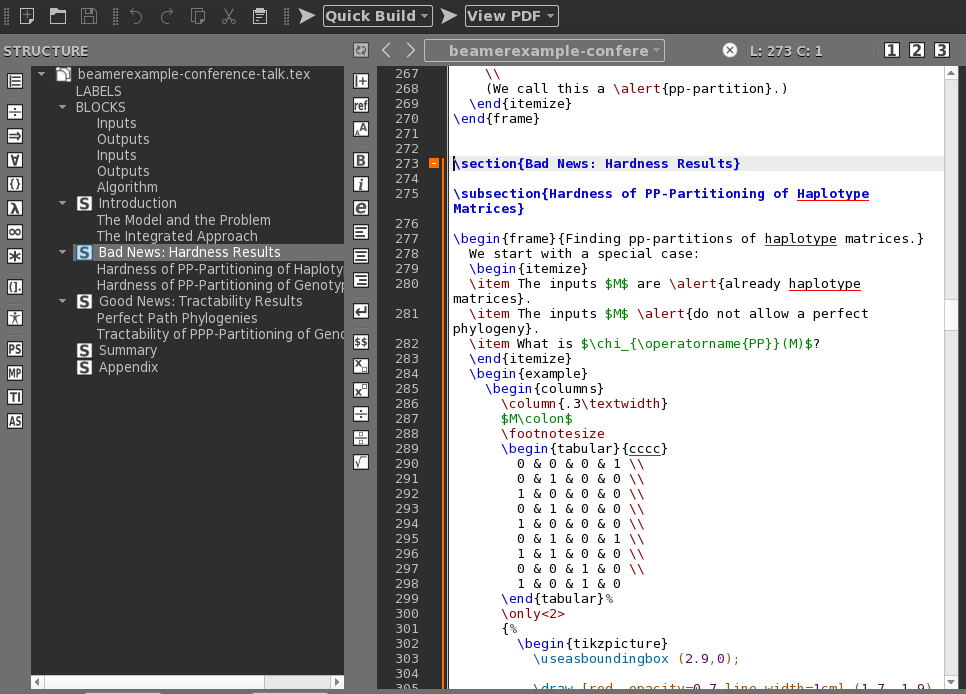
\includegraphics[width=0.99\linewidth]{../Norme_di_progetto/img/texMaker.png}
	\caption{\TeX{}maker - per la stesura dei documenti}
\end{figure}

\subsubsection{GanttProject}
GanttProject è un programma gratuito dedicato alla produzione dei diagrammi di Gantt\glo. Permette di creare task e milestone, organizzare le task in lavoro strutturato a interruzioni, disegnare
i vincoli di dipendenza tra di esse e molte altre utilità, generando automaticamente il relativo
diagramma. \\
\centerline{\url{https://www.ganttproject.biz/}}

\subsubsection{Draw.io}
Draw.io viene utilizzato per la produzione degli UML.\\
\centerline{\url{https://www.draw.io/}} 

\subsection{Gestione della configurazione}
L'obiettivo della configurazione è di creare ordine tra i documenti e il software. Tutto ciò che è configurato ha uno stato identificativo, è modificato secondo regole ben definite ed è posto sotto versionamento\glo.

\subsubsection{Versionamento}
\paragraph{Versionamento dei documenti} \mbox{} \\ \mbox{} \\
Ogni versione di qualsiasi documento deve corrispondere ad una riga della tabella delle modifiche. Il numero di versione è composto da tre cifre: \\ \\
\centerline{X.Y.Z} \\
\begin{itemize}
\item \textbf{X}: rappresenta una versione stabile del documento, resa tale dopo l'approvazione del \textit{Responsabile} di progetto: \begin{itemize}
\item inizia da 0 
\item viene incrementata di un'unità alla volta;
\end{itemize}
\item \textbf{Y}: indica l'ultima versione del documento che ha passato la fase di verifica: \begin{itemize}
\item inizia da 0;
\item viene incrementato dal verificatore ad ogni verifica;
\item quando viene incrementato X, viene riportato a 0.
\end{itemize} 
\item \textbf{Z}: indica l'ultima modifica apportata al documento dal redattore: \begin{itemize}
\item inizia da 0;
\item viene incrementato dal redattore del documento ad ogni modifica;
\item quando viene incrementato Y, viene riportato a 0.
\end{itemize}
\end{itemize}

\paragraph{GitHub} \mbox{} \\ \mbox{} \\
Per le parti del progetto da versionare si è scelto di usare GitHub\glo, un servizio del sistema di versionamento distribuito Git per contenere la repository remota. \\
I membri del team possono interagire con il VCS\glo sia da linea di comando, sia attarverso software che ne migliorano l'usabilità, come GitKraken e GitHub Desktop. La versione ufficiale del progetto è ospitata in una repository remota su GitHub, all'indirizzo \\
\centerline{\url{hhttps://github.com/teamafkSWE}}

\paragraph{Struttura del repository} \mbox{} \\ \mbox{} \\
All'interno della repository principale sopra descritta, ci sono due differenti repository: \begin{itemize}
\item \textbf{PredireConGrafana-docs}: contiene tutti i documenti ufficiali del progetto, suddivisi in specifiche cartelle: \\
\centerline{\url{https://github.com/teamafkSWE/PredireConGrafana-docs}}  \begin{itemize}
\item \textbf{Cartella principale - RR}: raccoglie i file sorgenti per la compilazione dei documenti, suddivisi tra esterni ed interni, realizzati per la \textit{Revisione dei Requisiti}. In futuro, saranno aggiunte cartelle distinte nominate \textbf{RP, RQ} e \textbf{RA}, contenenti i file delle rispettive consegne;
\begin{itemize}
\item[$\bullet$] \textbf{Tipologia\_di\_Documento}: ogni documento avrà la rispettiva cartella (e.i. Norme\_di\_Progetto), contenente tutti i file (sezioni ed immagini) necessari per la sua compilazione;
\item[$\bullet$] \textbf{copertina.tex}: file che permetterà una facile e rapida modifica dell'impostazione testuale del frontespizio;
\end{itemize}
\item \textbf{Template}: contiene tutti i file che definiscono il template \LaTeX{} per la creazione di nuovi documenti;
\end{itemize} 
\item \textbf{PredireConGrafana-SW}: conterrà tutti i file di codifica dei plug-in da sviluppare. \\ \centerline{\url{https://github.com/teamafkSWE/PredireConGrafana-SW}}
\end{itemize}
Entrambe le repository, avranno una propria struttura identica a livello: \begin{itemize}
\item \textbf{locale}: ogni membro del gruppo lavora sui file clonati dal repository remoto nel proprio PC;
\item \textbf{remoto}: presente su GitHub, contiene il lavoro svolto da ogni componente e che viene condiviso con il team.
\end{itemize}

\paragraph{Tipi di file} \mbox{} \\ \mbox{} \\
I file utilizzati per la documentazione del progetto sono: \begin{itemize}
\item file con estensione .tex di \LaTeX{};
\item file con estensione .pdf (da consegnare);
\item file di stile, .sty,  e immagini di supporto.
\end{itemize}
Il file ".gitignore" è presente al livello più esterno della repository ed elenca tutti i file esclusi dal versionamento.

\paragraph{Utilizzo di Git} \mbox{} \\ \mbox{} \\
Il repository di Git è composto da vari branch\glo, per favorire la collaborazione tra i vari membri e il parallelismo delle attività. Si consiglia quindi di seguire questa procedura:
\begin{enumerate}
\item scegliere il proprio branch di lavoro;
\item eseguire il pull\glo dal repository remoto, che effettua quindi l'aggiornamento del proprio repository locale;
\item svolgere il compito assegnato;
\item eseguire il comando di aggiunta (add) dei file nuovi o modificati da condividere all'area di staging\glo;
\item eseguire il comando di commit\glo dei file aggiunti, corredato da un messaggio che identifica il lavoro svolto;
\item eseguire il push\glo del commit sul repository remoto.
\end{enumerate}

\paragraph{Gestione delle modifiche}\mbox{} \\ \mbox{} \\
Tutti i membri del team possono modificare i file in ogni branch, ad eccezione del branch master, per il quale occorre richiedere una pull e ottenere l'approvazione di un altro membro.

\subsection{Gestione della qualità}
Lo scopo è di garantire che il prodotto e i servizi offerti rispettino gli obiettivi di qualità e che i bisogni del proponente siano soddisfatti. 

\subsubsection{Descrizione}
La gestione della qualità viene approfondita nel \textit{Piano di Qualifica}, dove sono descritte le modalità utilizzate per garantire la qualità nello sviluppo del progetto. In particolare: \begin{itemize}
\item sono presentati gli standard utilizzati;
\item sono individuati i processi\glo di interesse;
\item sono individuati gli attributi del software piè importanti per il progetto.
\end{itemize}
Per ogni processo vengono descritti: \begin{itemize}
\item gli obiettivi da perseguire;
\item le strategie da applicare;
\item le metriche da utilizzare.
\end{itemize}
L'obiettivo è quello di ottenere software e documentazione di qualità soddisfacente.

\subsubsection{Strumenti}
Gli strumenti utilizzati per la qualità sono:
\begin{itemize}
\item forniti dallo standard ISO-12207\footnote{ISO-12207: standard ISO per la gestione del ciclo di vita del software.};
\item le metriche.
\end{itemize}

\paragraph{Metriche} \mbox{} \\ \mbox{} \\
Le metriche sono distinte in tre categorie: processi, documentazione e codifica. Per ciascuna di esse si indica il motivo per cui è stata scelta e la procedura di calcolo.

\subparagraph{Classificazione}\mbox{} \\ \mbox{} \\
Le metriche rispetteranno la seguente notazione: \\
\centerline{\textbf{M[categoria][numero]}}
dove: \begin{itemize}
\item Categoria: indica la categoria della metrica, più precisamente:
\begin{itemize}
\item \textbf{P} per indicare le metriche dei processi;
\item \textbf{D} per indicare le metriche dei documenti;
\item \textbf{S} per indicare le metriche della codifica del software.
\end{itemize}
\item Numero: identifica in maniera univoca la metrica in ogni categoria, assume un valore intero a due cifre incrementale a partire da 1.
\end{itemize}
Se nelle formule di calcolo delle metriche è presente il simbolo "\#", va inteso come la parola "numero". Un esempio può essere il seguente:
\[ \#parole\_doc = numero\ di\ parole\ presenti\ nel\ documento \]
\pagebreak
\subparagraph{Metriche per i processi}  \mbox{} \\ 
\begin{table}[H]
\caption{Metriche dei processi}
	\begin{center}
	\begin{tabular}{ c | c | L{9.5cm} }
		\rowcolor{redafk}
		\textcolor{white}{\textbf{Nome}} & \textcolor{white}{\textbf{Codice}}& \centerline{\textcolor{white}{\textbf{Descrizione}}} \\
		Schedule Variance (SV)  & MP01 & La Schedule Variance indica se una certa attività o processo è in anticipo, in pari, o in ritardo rispetto alla data di scadenza prevista. \'E calcolata utilizzando la seguente formula: \newline
\[ SV = DCE-DCP\]
dove: \begin{itemize}
\item \textbf{DCE}: data conclusione effettiva;
\item \textbf{DCP}: data conclusione pianificata.
\end{itemize}
Se $SV \leq 0$ significa che l’attività o il processo è in pari o in anticipo, invece, se $SV > 0$ significa che l’attività è in ritardo. \\	
		Budget Variance (BV) & MP02 & Permette di controllare i costi sostenuti alla data corrente rispetto al budget preventivato. Viene calcolata in fase di consuntivo di periodo utilizzando la seguente formula: \newline
		\[ BV[\%] = \frac{CP-CE}{CE} \]		
dove: \begin{itemize}
\item \textbf{CP}: costo preventivato;
\item \textbf{CE}: costo effettivo.
\end{itemize}
Se $BV \geq 0$ indica che il budget sta venendo speso più lentamente di quanto pianificato, se negativo invece indica che il budget sta venendo speso più velocemente di quanto pianificato. \\
Produttività (P) & MP03 & Rappresenta la produttività media delle risorse impiegate, cioè delle persone coinvolte, nelle diverse fasi del progetto. E’ misurata in termini di numero di linee di codice (\hyperref[par:MS01]{LOC}) sviluppate da una persona nell’unità di tempo stabilita (settimana). E’utilizzata per valutare lo sforzo richiesto per lo sviluppo  del progetto a fronte delle sue dimensioni. 
\[ Pmedia = \frac{LOC}{settimana}\]
	\end{tabular}
	\end{center}
	\end{table}
\pagebreak
\subparagraph{Metriche per i documenti}\mbox{} \\ 
\begin{table}[H]
\caption{Metriche dei documenti}
	\begin{center}
	\begin{tabular}{ c | c | L{10cm} }
		\rowcolor{redafk}
		\textcolor{white}{\textbf{Nome}} & \textcolor{white}{\textbf{Codice}} & \centerline{\textcolor{white}{\textbf{Descrizione}}} \\
		Indice Gulpease (IG)  & MD01 & \'E un indice di leggibilità di un testo tarato sulla lingua italiana e basato su due variabili linguistiche: la lunghezza della parola e la lunghezza della frase rispetto al numero delle lettere. La formula per il suo calcolo è: \newline
\[ IG = 89 + \frac{300 \cdot (\#frasi) - 10 \cdot (\#lettere)}{\#parole} \] \newline
Il risultato è un valore compreso nell'intervallo tra 0 e 100, dove il valore 100 indica la più alta leggibilità. Un indice inferiore a 80 indica documenti di difficile leggibilità per chi ha la licenza elementare, inferiore a 60 per chi ha la licenza media, inferiore a 40 per chi ha un diploma superiore.
	\\
	\end{tabular}
	\end{center}	
	\end{table}
\pagebreak
\subparagraph{Metriche per la codifica} \mbox{} \\ \mbox{} \\
Questa sezione ha lo scopo di fornire delle metriche per garantire un buon livello di qualità del software.
\begin{table}[H]
	\caption{Metriche del software}
	\begin{center}
	\begin{tabular}{ C{4.5cm} | c | L{9.5cm} }
		\rowcolor{redafk}
		\textcolor{white}{\textbf{Nome}} & \textcolor{white}{\textbf{Codice}} & \centerline{\textcolor{white}{\textbf{Descrizione}}} \\
		\label{par:MS01}Linee di Codice (LOC) & MS01 & Rappresenta  le  dimensioni  del  codice  sorgente  (di  tutto  il  prodotto  software oppure di quello sviluppato in una versione specifica). \'E espresso in termini di numero di linee di codice, ed è utilizzato per dimensionare la produttività delle persone e da questa lo sforzo richiesto per sviluppare il prodotto. \\
		Numero dei Metodi (NM)  & MS02 & Numero medio di metodi contenuti nelle classi di un oggetto. Un numero troppo alto di metodi può indicare la necessità di scomporre la classe. Un numero troppo basso deve far riflettere sull'effettiva utilità della classe in esame. 
		\[ NM =\frac{\sum\#metodi}{\#classi}  \] \\
		Numero di Parametri (NP) & MS03 & Numero di parametri passati a un metodo. Un eccessivo numero di parametri passati ad un metodo può
indicare un’eccessiva complessità dello stesso. \\
		Commenti per Linee di \newline Codice (CLC) & MS04 & Rapporto fra numero di righe di commento e numero totale di righe (vuote escluse). Un codice ben commentato può essere compreso più facilmente e velocemente, facilitando le operazioni di manutenzione. 
		\[ CLC = \frac{\#righe\_commento}{\#tot\_righe}\] \\
		Code Coverage (CC) & MS05 & Percentuale delle linee di codice coperte dai test. Avere codice coperto da test riduce la possibilità di introdurre errori nel prodotto. 
		\[ CC[\%] = \frac{\#righe\_codice\_testate}{\#tot\_righe\_codice}\] \\
	\end{tabular}
	\end{center}
	\end{table}
\pagebreak
\subsubsection{Verifica}
Il processo di verifica ha come scopo la realizzazione di prodotti corretti, coesi e completi. Sono soggetti a verifica i documenti e il software.
Il processo di verifica deve rispettare i seguenti punti: \begin{itemize}
\item la verifica deve essere effettuata seguendo procedure ben definite;
\item per verificare vi sono criteri chiari e affidabili;
\item ogni fase del prodotto viene verificata;
\item dopo la verifica il prodotto è in uno stato stabile;
\item il prodotto può essere validato.
\end{itemize}
Il processo di verifica prende in input ciò che è già stato prodotto e lo restituisce in uno stato
conforme alle aspettative (stabile). Per ottenere tale risultato ci si affida a processi di analisi e test.
\paragraph{Strumenti di verifica}

\paragraph*{Correzione ortografica} \mbox{} \\ \mbox{} \\
Il controllo ortografico viene eseguito principalmente basandosi sugli strumenti integrati in \TeX{}maker, il quale fornisce un dizionario italiano e sottolinea in rosso le parole che non vi appartengono. 

\paragraph{Analisi} \mbox{} \\ \mbox{} \\
Il processo di analisi si suddivide in statica e dinamica.

\paragraph*{Analisi statica} \mbox{} \\ \mbox{} \\
L'analisi statica effettua controlli su documenti e codice. Questo tipo di analisi serve per rilevare varie tipologie di anomalie. \\
Questa attività viene effettuata con l'ausilio di due metodi manuali di lettura (attuati da persone) differenti: \begin{itemize}
\item \textbf{Walkthrough}: i vari componenti del team effettuano una lettura scrupolosa di documenti e/o codice alla ricerca di errori, senza sapere inizialmente se ce ne siano;
\item \textbf{Inspection}: i verificatori usano liste di controllo (checklist) per fare ispezione cercando errori specifici in parti specifiche. Questa tecnica permette quindi di aumentare l'efficienza dello sviluppo, diminuendo i tempi dell'analisi statica.
\end{itemize}
A seguire sono descritte le liste di controllo utilizzabili per le ispezioni:
\begin{table}[H]
\caption{Errori frequenti nei documenti}
\begin{center}
\begin{tabular}{C{4cm} | C{12cm}}
\rowcolor{redafk}
\textcolor{white}{\textbf{Oggetto}} & \centerline{\textcolor{white}{\textbf{Controllo}}} \\
Formato data & Deve seguire il formato gregoriano YYYY-MM-DD \\
Sintassi & La frase è troppo complessa e deve essere semplificata \\
Punteggiatura degli elenchi & Ogni voce termina in ";" eccetto l'ultima che termina in "."\\
Errori di battitura & Tipici errori di battitura dovuti alla vicinanza delle
lettere sulla tastiera, ad esempio la lettera "a" al posto della "s", "i" al posto di "o", "m" al posto di "n" \\
Gerarchia delle sezioni & Non viene scritta la gerarchia delle sezioni dei documenti in maniera adeguata, ovvero: section, subsection, subsubsection, paragraph, subparagraph
\end{tabular}
\end{center}
\end{table}

\paragraph*{Analisi dinamica} \mbox{} \\ \mbox{} \\
L'analisi dinamica è una tecnica di analisi del prodotto software che richiede la sua esecuzione. Produce una misura della qualità del prodotto, mediante l'esecuzione di test specifici che verificano se il prodotto funziona e se ci sono anomalie.

\paragraph{Test} \mbox{} \\ \mbox{} \\
I test sono l'attività fondamentale dell'analisi dinamica: il loro scopo è verificare che il codice
scritto funzioni correttamente. I test devono:
\begin{itemize}
\item essere ripetibili;
\item specificare l'ambiente di esecuzione;
\item identificare input e output richiesti;
\item avvertire di possibili effetti indesiderati;
\item fornire informazioni sui risultati dell'esecuzione.
\end{itemize}
Ci sono vari tipi di test, ognuno dei quali ha un diverso oggetto di verifica e scopo.

\paragraph*{Test funzionali} \mbox{} \\ \mbox{} \\
Test condotti per valutare la conformità di un componente o sistema con requisiti\glo funzionali. Ne fanno parte: \begin{itemize}
\item \textbf{Test di unità\glo}: si eseguono su unità di software, e si concentrano sul loro funzionamento individuale;
\item \textbf{Test di integrazione}: verificano se sono rispettati i contratti di interfaccia tra più moduli o sub-system (interni o esterni);
\item \textbf{Test di accettazione UAT}: gli UAT (User Acceptance Testing) si occupano di verificare il prodotto e, in particolare, il soddisfacimento del cliente. Il superamento di questo test garantisce che il software sia pronto per essere rilasciato.
\end{itemize}

\paragraph*{Test di regressione} \mbox{} \\ \mbox{} \\
Il test di regressione va eseguito ogni volta che viene modificata un’implementazione in un programma. È possibile eseguire nuovamente i test esistenti sul codice modificato, integrando solo le parti che abbiano precedentemente superato il test di unità, per stabilire se le modifiche apportate hanno alterato elementi precedentemente funzionanti.\\ Se necessario è anche possibile scrivere nuovi test.

\paragraph*{Test di sistema} \mbox{} \\ \mbox{} \\
Verificano il comportamento dell'intero sistema.\\
Lo scopo principale di questi test è la verifica del sistema rispetto alle specifiche tecniche definite nell'\textit{Analisi dei Requisiti}.

\subsubsection{Validazione}
Questo processo avviene tramite test pianificati dal \textit{Progettista} ed in seguito eseguiti dal \textit{Verificatore}.
Lo scopo di quest'ultimi è appunto accertare che il prodotto finale corrisponda alle attese, soddisfando tutti i requisiti concordati e i bisogni del committente. \\
Tali test sono soggetti a tracciamento e verranno riportati all'interno del \textit{Piano di Qualifica}.

\pagebreak
	
\section{Processi Organizzativi}

\subsection{Gestione di Progetto}

\subsubsection{Ruoli di progetto}
Ciascun membro del gruppo, a rotazione, deve ricoprire il ruolo che gli viene assegnato e che corrisponde all'omonima figura aziendale. Nel \textit{Piano di Progetto}\glo vengono organizzate e pianificate le attività assegnate agli specifici ruoli. I ruoli che ogni componente del gruppo è tenuto a rappresentare sono descritti di seguito.

\paragraph{Responsabile di progetto}\mbox{} \\ \mbox{} \\
Il \textit{Responsabile di progetto} (o semplicemente \textit{Responsabile}) è una figura chiave in quanto ricadono su di lui le responsabilità di pianificazione, gestione, controllo e coordinamento delle risorse e attività del gruppo. Il \textit{Responsabile} si occupa anche di interfacciare il gruppo con le persone esterne facendo da intermediario: sono quindi di sua competenza le comunicazioni con committente e proponente.
Questa figura è incaricata anche di analizzare e gestire le criticità, che si incontrano durante il progetto, e di approvare i documenti.

\paragraph{Amministratore di progetto}\mbox{} \\ \mbox{} \\
L'\textit{Amministratore} ha il compito di supporto e controllo dell'ambiente di lavoro.
Egli deve quindi:
\begin{itemize}
	\item dirigere le infrastrutture di supporto;
	\item risolvere problemi legati alla gestione dei processi;
	\item gestire la documentazione;
	\item controllare versioni e configurazioni.
\end{itemize}

\paragraph{Analista}\mbox{} \\ \mbox{} \\
L'\textit{Analista} si occupa di analisi dei problemi e del dominio applicativo. Questa figura ha anche il compito di redigere i documenti, in questo caso può essere definito come \textit{Redattore}.
Le sue responsabilità sono:
\begin{itemize}
	\item studio del dominio del problema;
	\item definizione della complessità e dei requisiti dello stesso;
	\item redazione del documenti:\textit{ Analisi dei Requisiti} e \textit{Studio di Fattibilità}.
\end{itemize}

\paragraph{Progettista}\mbox{} \\ \mbox{} \\
Il \textit{Progettista} gestisce gli aspetti tecnologici e tecnici del progetto.
Il \textit{Progettista} deve:
\begin{itemize}
	\item effettuare scelte efficienti ed ottimizzate su aspetti tecnici del progetto;
	\item sviluppare un'architettura che sfrutti tecnologie note ed ottimizzate, su cui basare un prodotto stabile e manutenibile.
\end{itemize}

\paragraph{Programmatore}\mbox{} \\ \mbox{} \\
Il \textit{Programmatore} è responsabile della codifica del progetto e delle componenti di supporto che serviranno per effettuare le prove di verifica e validazione sul prodotto.
Il \textit{Programmatore} si occupa di:
\begin{itemize}
	\item implementare le decisioni del progettista;
	\item creare o gestire componenti di supporto per la verifica e validazione del codice.
\end{itemize}

\paragraph{Verificatore}\mbox{} \\ \mbox{} \\
Il \textit{Verificatore} si occupa di controllare il prodotto del lavoro svolto dagli altri membri del team, sia esso codice o documentazione. Per le correzioni si affida agli standard definiti nelle \textit{Norme di Progetto}, nonché alla propria esperienza e capacità di giudizio.
Il \textit{Verificatore} deve:
\begin{itemize}
	\item ispezionare i prodotti in fase di revisione, avvalendosi delle tecniche e degli strumenti definiti nelle \textit{Norme di Progetto};
	\item evidenziare difetti ed errori del prodotto in esame;
	\item segnalare eventuali errori trovati all'autore dell'oggetto preso in esame o alla persona che ha responsabilità su di esso.
\end{itemize}

\subsubsection{Gestione dei rischi}
È compito del \textit{Responsabile} rilevare i rischi e renderli noti, tramite un continuo monitoraggio e una continua identificazione di quest'ultimi. \\
Qualora dovesse essere \textbf{identificato} un nuovo rischio è necessario procedere con i seguenti passaggi:
\begin{enumerate}
	\item \textbf{Classificare} il rischio seguendo la codifica;
	\item \textbf{Descrivere} una strategia da applicare per gestire il rischio;
	\item \textbf{Riportare} il rischio nel \textit{Piano di Progetto}.
\end{enumerate}

\paragraph{Codifica}\mbox{} \\ \mbox{} \\
La codifica dei rischi è utilizzata per la classificazione. Il codice di un rischio si presenta nella forma: \\
\centerline{\textbf{Ri[Categoria][Grado][Numero]}}
dove:
\begin{itemize}
	\item \textbf{Categoria}: indica la categoria del rischio, essa può assumere i valori:
	\begin{itemize}
		\item \textbf{O} per i rischi organizzativi;
		\item \textbf{T} per i rischi tecnologici;
		\item \textbf{P} per i rischi interpersonali.
	\end{itemize}
	\item \textbf{Grado}: indica il grado di rischio, è la somma tra la probabilità e la gravità. Queste ultime possono assumere i seguenti valori:
	\begin{itemize}
		\item \textbf{0}: bassa;
		\item \textbf{1}: media;
		\item \textbf{2}: alta.
	\end{itemize}
	(In questo caso un rischio con una probabilità bassa ma una gravità alta avrà lo stesso grado di un rischio con una probabilità alta e una gravità bassa, ovvero 2)
	\item \textbf{Numero}: insieme a categoria e grado identifica in maniera univoca il rischio, può assumere un valore intero progressivo ad una cifra (0-9).
\end{itemize}

\subsection{Processi di Coordinamento}
Di seguito vengono descritte le norme che regolano le comunicazioni e gli incontri del gruppo, che siano tra i membri o con committenti e proponenti.
\subsubsection{Gestione Comunicazioni}
\paragraph{Comunicazioni Interne}\mbox{} \\ \mbox{} \\
Le comunicazioni interne ai membri del gruppo vengono gestite  tramite 2 applicazioni:
\begin{itemize}
	\item Telegram\glo;
	\item Discord\glo.
\end{itemize}
È stato disposto un gruppo Telegram sul quale si discute di tematiche generali o collettive, garantendo risposte rapide e ordinate in caso di decisioni per votazione, grazie ad apposite funzioni dette bot di Telegram\glo. \\
Discord viene usato principalmente per le riunioni tra i membri del gruppo, ma l'applicazione mette anche a disposizione dei canali testuali. Tali canali sono stati suddivisi per tema e vengono usati per le comunicazioni specifiche per agevolare la stesura dei documenti. Vengono suddivisi in:
\begin{itemize}
	\item \textbf{General}: per discussioni riguardanti rotazioni dei ruoli e decisione degli argomenti da discutere nelle riunioni;
	\item \textbf{Links}: per tenere traccia di tutti i link utili al progetto;
	\item \textbf{Analisi-requisiti}: per discutere gli Use Case\glo e i requisiti necessari alla stesura dell'\textit{Analisi dei Requisiti};
	\item \textbf{Norme}: per discutere riguardo le regole del \textit{Way of Working} del gruppo, le norme da seguire e, di conseguenza, la stesura del documento \textit{Norme di Progetto}\glo;
	\item \textbf{Piano-progetto}: per confrontarsi riguardo il monte ore dei vari ruoli e per facilitare la stesura del documento \textit{Piano di Progetto};
	\item \textbf{Piano-qualifica}: per discutere di strategie da attuare per garantire qualità attraverso verifica\glo e validazione\glo.
\end{itemize}
\paragraph{Comunicazioni Esterne}\mbox{} \\ \mbox{} \\
Le comunicazioni con soggetti esterni al gruppo sono di competenza del responsabile. Gli strumenti predefiniti sono la posta elettronica, dove viene utilizzato l'indirizzo \href{mailto:gruppoafk15@gmail.com}{gruppoafk15@gmail.com}.
Per comunicare con \textit{Zucchetti SPA} viene usato il servizio Skype\glo per le chiamate. Il responsabile ha il compito di tenere informati gli altri componenti del gruppo in caso di assenza.

\subsubsection{Gestione Riunioni}
Le riunioni possono essere interne o esterne. All'inizio di ogni riunione il \textit{Responsabile} nomina, tra i componenti del gruppo, un \textit{Segretario} che si occuperà di far rispettare l'ordine del giorno. Inoltre ha l'onere della stesura del \textit{Verbale di Riunione}\glo.

\paragraph{Riunioni interne} \mbox{} \\ \mbox{} \\
E' compito del \textit{Responsabile} organizzare riunioni interne al gruppo. Ciò prevede, più nello specifico, la stesura dell'ordine del giorno e
stabilire data, orario e luogo di incontro, mediando se necessario con i membri per permettere la presenza di tutti. Le riunioni sono tenute principalmente usando Discord, così da essere il più facilmente raggiungibili.
Il \textit{Responsabile} deve inoltre assicurarsi, attraverso la comunicazione
mediante i mezzi propri del gruppo, che ogni componente sia pienamente a conoscenza della riunione in tutti i suoi dettagli. \\
D'altro canto ogni membro del gruppo deve presentarsi puntuale agli appuntamenti,
e comunicare in anticipo eventuali ritardi o assenze adeguatamente giustificate.

\paragraph{Riunioni esterne} \mbox{} \\ \mbox{} \\
E' nuovamente compito del \textit{Responsabile} organizzare riunioni esterne.
Nello specifico egli deve preoccuparsi di contattare l'azienda proponente per fissare gli
incontri e qualora sia necessario, tenendo conto anche delle preferenze di date e orario
espresse dagli altri membri del gruppo. La partecipazione a tali riunioni deve essere,
a meno di casi eccezionali, unanime.
Ogni membro del gruppo può, inoltre, esprimere al Responsabile una richiesta, adeguatamente motivata, di fissare una riunione esterna. A questo punto sarà compito
dello stesso Responsabile giudicare come valida o meno la richiesta presentatagli ed
agire di conseguenza.

\paragraph{Verbale di riunione} \mbox{} \\ \mbox{} \\
Ad ogni riunione, interna o esterna, è compito del \textit{Segretario} designato redigere il \textit{Verbale di riunione} corrispondente, che deve essere poi approvato dal \textit{Responsabile}. La struttura del \textit{Verbale} è definita in \hyperref[par:verbali]{§ 3.5.5}.


\subsection{Strumenti}
Il gruppo, nel corso del progetto, ha utilizzato o utilizzerà i seguenti strumenti:
\begin{itemize}
	\item \textbf{Telegram}: strumento di messaggistica usato per comunicazioni veloci tra i membri; 
	\item \textbf{Discord}: per comunicazioni specifiche o per riunioni interne;
	\item \textbf{Git}: sistema di controllo di versionamento;
	\item \textbf{Gitflow}: sistema per agevolare varie operazioni su Git;
	\item \textbf{GitHub}: per il versionamento e il salvataggio in remoto di tutti i file riguardanti il progetto;
	\item \textbf{GanttProject}: software OpenSource\glo usato per la realizzazione dei diagrammi di Gantt;
	\item \textbf{Google Doc}: editor di testo cloud, usato per tenere degli appunti modificabili da tutti;
	\item \textbf{Google Drive}: utilizzato per il salvataggio in remoto dei file non sottoposti a versionamento, in modo da essere reperibili a tutti i membri;
	\item \textbf{Google Calendar}: per tenere traccia delle varie scadenze o riunioni fissate;
	\item \textbf{Skype}: servizio che offre possibilità di fare videoconferenze e chiamate VoIP, utilizzato per comunicare con il proponente;
	\item \textbf{Sistema Operativo}: i requisiti non indicano la necessità di usare un sistema operativo specifico, verranno quindi utilizzati Windows, Linux e Mac OS dai diversi membri del team.
\end{itemize}
%\pagebreak

\end{document}